\section{Evaluation}
\label{sec:eval}

We evaluated \cheetah{} on an AMD Opteron machine, which has 48 cores and 128 GB memory. \todo{Each processor is a 4-core 64-bit Intel Xeon, operating at 1.6 GHz with a 4MB shared L2 cache a 32KB per-core L1 cache.}  We performed experiments on two well-known benchmark suites: Phoenix~\cite{phoenix-hpca} and PARSEC (with native input)~\cite{parsec}. Table~\ref{} shows the detailed description of each benchmark. 

We use gcc-4.6 to compile these benchmarks, with {\tt -O2} option. For Phoenix benchmarks, we run them using 16 threads because these benchmarks often have too small working set. For PARSEC benchmarks, we run them with 48 threads. Since \cheetah{} is based on the sampling technique, running with more threads will generally runs too fast. We need to run a benchmark at least 5 second to get enough statistical samples. \\

\sloppy{}
Our evaluation will answer the following research questions in order as follows. 

\begin{itemize}
\item How effective can \cheetah{} find existing false sharing problems? How helpful are those information to fix false sharing problems?  (Section~\ref{sec:effectiveness})

\item What is the performance overhead of \cheetah{}? (Section~\ref{sec:perf})

\item How is the precision of assessment?  (Section~\ref{sec:precision})

\end{itemize}

\subsection{Effectiveness}
\label{sec:effectiveness}

\cheetah{} detects two existing false sharing problems, \texttt{linear\_regression} in Phoenix and \texttt{streamcluster} in Parsec, which has been discovered by prior work~\cite{Sheriff, Predator}. In the remaining of this section, we discuss how reported information can help us to confirm and fix these false sharing problems. 

%Finally, we study the false sharing that \cheetah{} does not detect in these benchmarks and verify that they have negligible impact to the overall program execution. 

\subsubsection{linear\_regression}
Figure~\ref{fig:lr} shows the output of \cheetah{}. It points out that the {\tt tid\_args} object allocated at line 139, with the structure type {\tt lreg\_args}, incurs a severe false sharing problem. According to our assessment, fixing it can possibly improve the performance by $5.7\times$, where the assessment precision is further discussed in Section~\ref{sec:precision}. By examining the source code, we can discover that the {\tt tid\_args} object is passed to different threads linear\_regression\_pthread. Then we can easily find out where false sharing has been exercised, which is shown as Figure~\ref{lr:code}. By checking the word-based information which is not shown in the Figure~\ref{fig:lr}, we can understand the reason of this false sharing problem: different threads are updating different parts of the object {\tt tid\_args} simultaneously, where each thread updates the size of the structure lreg\_args of this common array. This problem is exactly the same as that shown in Figure~\ref{fig:fsinfs}. 

To address the problem, we pad the structure {\tt lreg\_args} with extra bytes, by adding 64 bytes useless content, so that we can force different threads not to access the same cache line. The simple optimization lead to a 5.7$\times$ speedup, which matches the assessment 5.76$\times$ given by \cheetah{}.

\begin{figure}
\begin{minipage}{\columnwidth}

\centering

\fbox
{
\begin{minipage}{3in}
Detecting a false sharing at object: start 0x400004b8 end 0x400044b8 (with size 4000).  Accesses 1263 invalidations 27f writes 501 total latency on this object was 102988 cycles.

Latency information: totalThreads 16 totalThreadsAccesses 12e1 totalThreadsCycles 106389 longestRuntime 7652 threadReduceRate 0.164697 totalPossibleImprovementRate 576.172748\% (realRuntime 7738 predictedRuntime 1343).

It is a heap object with the following callsite:
linear\_regression-pthread.c: 139
\end{minipage}
}
\vspace{1em}
\caption{The output of \cheetah{} for Linear\_Regression.}
\label{fig:lr}
\end{minipage}
\end{figure}


\begin{figure}
\begin{verbatim}
typedef struct
{
  ......  
  long long SX;
  long long SY;
  long long SXX;
  ......
} lreg_args;	

for (i = 0; i < args->num_elems; i++)
{
  //Compute SX, SY, SYY, SXX, SXY
  args->SX  += args->points[i].x;
  args->SXX += args->points[i].x
              *args->points[i].x;
  args->SY  += args->points[i].y;
  ......
}
\end{verbatim}
\caption{The data object and the structure type that cause false sharing.}
\label{lr:code}
\end{figure}

\subsubsection{streamcluster}

%Figure~\ref{fig:sc} shows the output of StreamCluster. 
Inside the streamcluster, every thread will update the work\_mem heap object concurrently, located in line 985. The authors have already added some padding to avoid false sharing. However, the size of cache line (as a macro) is set to be 32 bytes, which is smaller than the size of actual cache line used in our experimental machine. Thus, streamcluster will has a significant false sharing problem. The performance impact of fixing false sharing problems inside is further discussed in Section~\ref{sec:precision}. 


\subsubsection{Comparing with state-of-the-art}

\begin{figure}[htbp]
\centering
\label{fig:fseffectiveness}
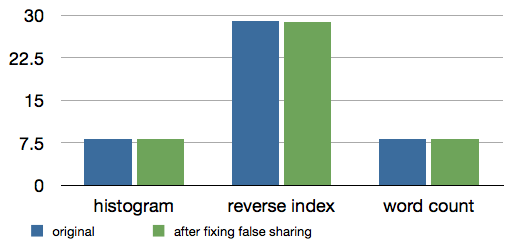
\includegraphics[width=.8\columnwidth]{figure/trivial}
\caption{False sharing problems missed by \cheetah{} have negligible performance impact.}
\end{figure}

%\cheetah{} may miss some false sharing instances because of its sampling feature. 
\cheetah{} can only detect false sharing problems that actually occur in the execution. As observed by Predator~\cite{Predator}, the occurrence of false sharing can be affected by the starting address of objects or the size of the cache line. \cheetah{} may also miss false sharing instances if the number of accesses on them is not significant enough, because of \cheetah{}'s sampling feature. In this section, we will compare \cheetah{}'s effectiveness with the state-of-the-art tool -- Predator~\cite{Predator}, which observes the largest number of false sharing instances. 

Comparing with Predator, \cheetah{} can not detect false sharing problems in the histogram, reverse\_index, and word\_count. We fixed false sharing problems inside based on Predator's detection and ran these applications on our hardware \todo{with XXX threads}, with and without false sharing problems. Figure~\ref{fig:fseffectiveness} shows the performance impact of fixing false sharing: that all these benchmarks do not show a significant speedup after fixes, with less than 0.1\% improvement.  

\subsection{Performance Overhead}
\label{sec:perf}

\begin{figure*}[htbp]
\centering
\label{fig:overhead}
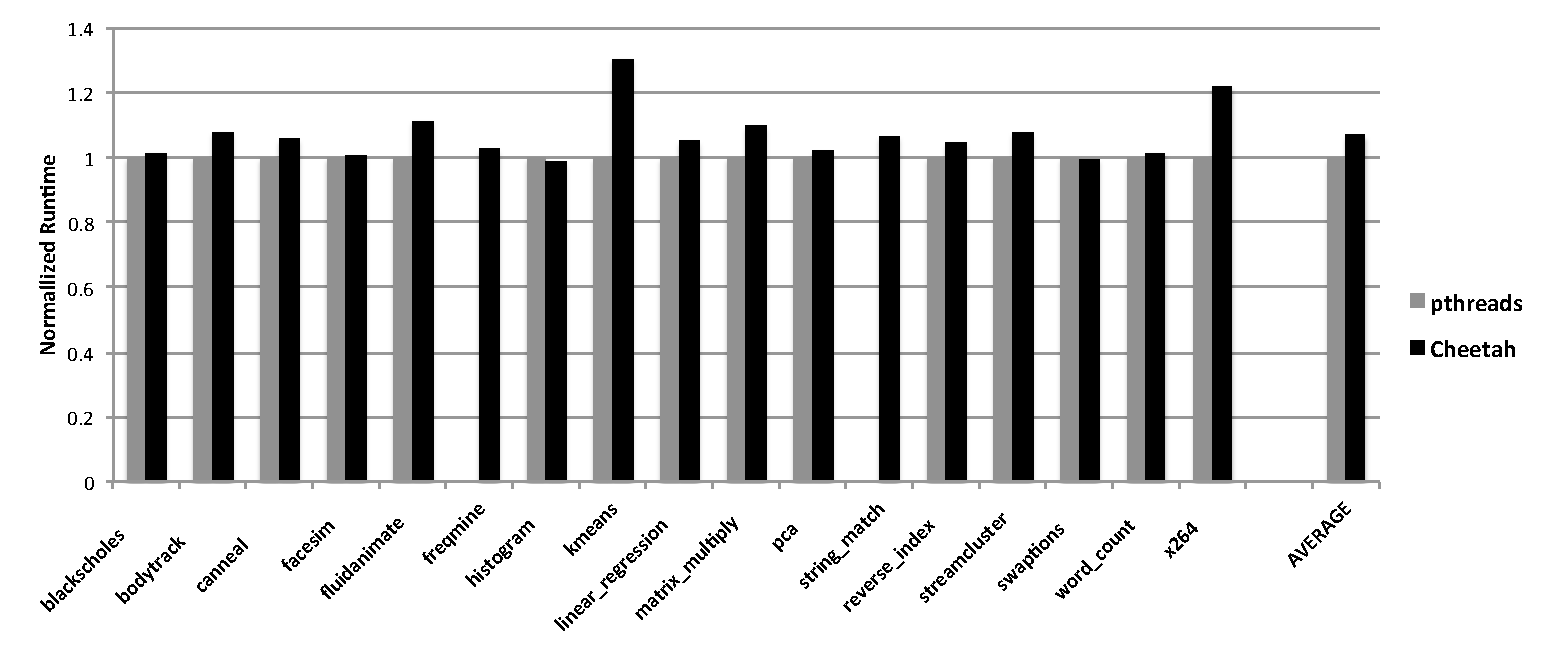
\includegraphics[width=2\columnwidth]{figure/Overhead.pdf}
\caption{Runtime overhead of \Cheetah{}. We normalized the runtime to that of \pthreads{}. Averagely, \cheetah{} only introduces around 7\% performance overhead on all evaluated benchmarks, which makes it practical to be used in the deployed software. }
\end{figure*}

We show the runtime overhead of \cheetah{} in Figure~\ref{fig:overhead}. We evaluated all benchmarks for three times and shown the average results here. According to this figure, \cheetah{} only introduces around 7\% performance overhead, which makes it practical to be utilized in the real deployment. 

We configure \cheetah{} with the sampling frequency at 64K instructions. Thus, for every 64K instructions, the pre-installed trap handler will be notified once so that \cheetah{} can collect the information of each sampled memory access. Because of \cheetah{}'s very coarse sampling rate, we should  let programs to run sufficiently long enough for our tool. If an application only runs less than 5 seconds, \cheetah{} can not gather enough data for the detection and assessment. Thus, we changed all phoenix benchmarks to only create 16 threads for each application, even the hardware has 48 cores.  We created 16 threads for Parsec benchmarks too, if arguments includes the number of threads. For other benchmarks, we used 48 threads. 

The performance overhead of \cheetah{} mainly comes from the following aspects. 
\paragraph{Sampling overhead.} When there is a sample, we have to collect information about this access, such as the type of access (read or write) and the number of cycles. We will update the history table of its corresponding cache line.

\paragraph{Thread creation overhead.} For each thread creation, \cheetah{} will initialize thread related data structure, get the timestamp, and record phase related information. Thus, for an application with a large number of threads, such as kmeans, \cheetah{} introduces slightly more overhead. 

 \todo{Should we check how the performance overhead will be changed at a different sample frequency?}

\subsection{Assessment Precision}
\label{sec:precision}

Different with previous tools, \cheetah{} can assess the performance impact of false sharing problems so that programmers can focus only on important problems. This section evaluates the precision of assessment. 

We evaluated the precision of assessment on two applications, \texttt{linear\_regression} and \texttt{streamcluster}, since they have been observed to have serious false sharing problems. We listed the results as Table~\ref{tbl: precision}. In this table, \texttt{linear\_regression} is abbreviated as ``linear\_rg''.  We evaluated different situations for these two cases, when the number of threads is equal to 16, 8, 4, and 2 correspondingly. We listed the predicted performance impact in the ``Assessment'' column and the actual improvement in the ``Real Case'' column of the table. 

Results of Table~\ref{tbl: precision} show that \cheetah{} can perfectly assessment the performance impact of false sharing in every case. Relying on the assessment, programmers don't have to spend time on those in-significant false sharing problems any more. 


\begin{table}
  \small
  \centering
  \begin{tabular}{ c | c | c | c}
  \textbf{Application} & {Threads (\#)} & \textbf{Assessment} & \textbf{Real Case} \\ \hline
\texttt{linear\_re} & 16 & 6.44X    & 6.7X \\
\texttt{linear\_re}& 8  & 5.56X    & 5.4X \\
\texttt{linear\_re} & 4  & 3.86X  & 4.1X  \\
 \texttt{linear\_re}& 2  & 2.18X  & 2X    \\ \hline
 \texttt{streamcluster} & 16 & 1.016X    & 1.015X \\
 \texttt{streamcluster} & 8 & 1.017X    & 1.018X \\
 \texttt{streamcluster} & 4 & 1.024X    & 1.022X \\
 \texttt{streamcluster} & 2 & 1.033X    & 1.035X \\
\end{tabular}
  \caption{
    Precision of assessment. \label{tbl: precision}}
\end{table}